\makeatletter
\def\@makeschapterhead#1{%
  \vspace*{10\p@}%
  {\parindent \z@ \centering \normalfont
      {\includegraphics[scale=1]{om.eps}}\\[10pt]
      {\Large\bf shirxV shirxVraMga sadugxraveV namaH}\\[10pt]
      %\par\nobreak
      %\vskip 5\p@    
    \interlinepenalty\@M
    \huge \bfseries  #1\par\nobreak
    \chaptermark{#1}
    \vskip 20\p@
  }}
\makeatother

\chapter*{parxkAshakara nuDi}

{\addTOCLine{parxkAshakara nuDi}}

shirxVraMga mahAgurugaLa parxvacanagaLa saMkalanavAda amaravANiV 11 neya\break \hbox{saMpuTa} ``saMsakxqqta-saMsakxqqti" eMba garxMthada karaDuparxtiyanunx utAthxna dAvxdashi\-yaMdu shirxVmAteyavarige samapaRNe mADi, avara AshiVvARda paDedu iMdu mudirxtarUpadalilx janateya muMdiDalu saMtoVSisutetxVve.

shirxV guruBagavaMtaru kuLitAga, niMtAga, reYlinalilx parxyANa mADutitxdAdxga, BoVjanada samayadalilx parxshenxgaLaninxTATxga, nAvugaLu sikikxdAga namamxgaLa shikaSxNakAkxgi saMsakxqqtige saMbaMdhisida mAtugaLanunx ADutatxleV idadxru. navarAtirxkAladalilx, beVsige rajadalilx elalxrU oTiTxge seVridAga (samemxVLanagaLalilx) basariVkaTeTxya sadugxru vidAyxshAleyalilx pATharUpavAgi parxvacanagaLanUnx anugarxhisidUdx uMTu. aneVka pATha parxvacana\-gaLanunx keVLidadxrU, avara vicAradhAreyanunx garxhisalu kaSaTxvAgutitxdudxdariMda, oMdu cwkaTiTxnalilx pATha\-gaLanunx namage iTaTxre, namage garxhisalu sulaBavAgutatxdeMba pArxthaRneyanunx nAnomemx iTATxga tatAkxla\-dalelxV mUlaBUtavAda viSayagaLa bagegx hinenxle pAThavanAnxraMBisidaru. sUkxlu, kAleVju, APiVsu\-gagaLalilx hAgU saMsakxqqtapATha shAleyalilx kelasamADutitxdadx namamxgaLa virAma kAlagaLalilx aMdare shani\-vAra, BAnuvAra, hAgU sAvaRtirxka rajAdinagaLu- pAThashAlege anadhayxyana rajAdinagaLu oTiTxge seVri baMdAga, pAThagaLanunx muMduvarisuva yoVjane sidadhxvAyitu.  kelavu hiriya sadasayxranunx Ayekx mADikoMDu avarugaLige pAThavaninxTuTx avariMda itara sadasayxrige pAThaviDisabeVkeMbudU I yoVja\-neya aMgavAyitu. idaraMte naDeda kelavu mUlaBUta pAThagaLanuynx `` ASaRvideyxgaLa mwlikate" eMba shiVSiRkeyalilx I saMpuTadalilx koDalAgide. I pAThagaLigeV seVrida `dashaRna' (``jiVvana\-dalilxya noVTa") eMba pAThavu amaravANiV 1neya saMpuTadalilx `jiVvana dashaRna' eMba shiVSiRkeyalilx acAcx\-giruvudariMda matetx I saMpuTadalilx adanunx seVrisilalx.

saMsakxqqta AyoVgada parxshAnxvaLige kaLuhisida utatxra hAgU shirxVmanamxhArAja jayacAmarAjeVMdarx oDeyaravaru keVLidadx parxshenxgaLige koTaTx utatxragaLu, saMsakxqqtige saMbaMdhisida aneVka mwlika saMgatigaLanunx oLagoMDiruvudariMda, avugaLanUnx I saMpuTadalilx seVrisalAgide.

namamx saMsethxge modalige `vijAcnxna maMdira' eMdu hesaranunx shirxVguruBaga\break\-vaMtaru koTiTxdadxru. `vijAcnxna'da hiMde `aSATxMgayoVga' (jAcnxna) ideyeMbu\-danunx tiLisutitxdadxru. I parxvacanagaLalilx maMdira\-vanunx `vijAcnxnamaMdira' eMdeV ulelxVKiside. maMdiravanunx 1968 ralilx rijisaTxrf mADisuvAga ``aSATxMgayoVga vijAcnxna maMdiraM" eMba pUNaRvAda hesaranunx baLasalu shirxV gurudeVvaru anumati koTaTxru.

noVTusx hAgU mUlabarahagaLanunx parishiVlisi, I saMpuTadalilxna leVKana\-gaLanunx acicxgAgi sidadx\-paDisi, aneVka saMsakxqqta mUlagaLige kananxDa BAvAnuvAda\-vanunx niVDi hAgU I saMpuTakekx BUmike\-yanUnx saha barediruva namamx hiriya soVdara vidAvxnf enf. esf. rAmaBadArxcAyaRrige namamx kaqtajacnxtegaLu. I saMpuTada parxkAshanadalilx neravu niVDiruva vidAvxnf enf. esf. janAdaRnAcArayxru, iMDekfsx sidadhx\-paDisuvudu, sholxVkagaLige BAvAnuvAda itAyxdiyAgi parxkAshanadalilx udadxkUkx neravu niVDi\-ruva DA|| ke. elf. shaMkaranArAyaNa joVyisaru, citarxvoMdanunx baredukoTuTx seVve salilxsiruva ci|| haSaR siMha, savxlapxmaTiTxge AthiRka neravu niVDi, garxMthada beleyanunx kaDimeyAgiyeV iDalu sAdhayx\-vAguvaMte mADiruva soVdara ji. ke. shirxVnivAsamUtiR hAgU otAtxse niVDutitxruva maMdirada soVdara-\-soVdari vagaR-ivarelalxrigU kaqtajacnxtegaLu.

aMdavAgi mudarxNa mADi, sahakAra niVDiruva caMcu perxsisxna shirxV Arf. narasiMha avaru namamx kaqtajacnxtege pAtarxru.

elalxdakUkx migilAgi, namage sUPxtiR cilumeyAgi namamxnunx anugarxhisi huri\-duMbisutitxruva paramapUjayx vijayalakiSxmXV shirxVmAteyavarige pArxNa parxNAmagaLu.

\vskip 1cm

\noindent Ishavxra saMvatasxra \hfill shaMkaranArAyaNadAsa

\noindent veYshAKa shukalx EkAdashiV \hfill (shirxVkaMTha)

\noindent {(\rm 18--5--1997)} \hfill kAyaRdashiVR

